\documentclass[handout,nooutcomes, noauthor]{ximera}

\title{Home Base}

\usepackage{gensymb}
\usepackage{tabularx}
\usepackage{mdframed}
\usepackage{pdfpages}
%\usepackage{chngcntr}

\let\problem\relax
\let\endproblem\relax

\newcommand{\property}[2]{#1#2}




\newtheoremstyle{SlantTheorem}{\topsep}{\fill}%%% space between body and thm
 {\slshape}                      %%% Thm body font
 {}                              %%% Indent amount (empty = no indent)
 {\bfseries\sffamily}            %%% Thm head font
 {}                              %%% Punctuation after thm head
 {3ex}                           %%% Space after thm head
 {\thmname{#1}\thmnumber{ #2}\thmnote{ \bfseries(#3)}} %%% Thm head spec
\theoremstyle{SlantTheorem}
\newtheorem{problem}{Problem}[]

%\counterwithin*{problem}{section}



%%%%%%%%%%%%%%%%%%%%%%%%%%%%Jenny's code%%%%%%%%%%%%%%%%%%%%

%%% Solution environment
%\newenvironment{solution}{
%\ifhandout\setbox0\vbox\bgroup\else
%\begin{trivlist}\item[\hskip \labelsep\small\itshape\bfseries Solution\hspace{2ex}]
%\par\noindent\upshape\small
%\fi}
%{\ifhandout\egroup\else
%\end{trivlist}
%\fi}
%
%
%%% instructorIntro environment
%\ifhandout
%\newenvironment{instructorIntro}[1][false]%
%{%
%\def\givenatend{\boolean{#1}}\ifthenelse{\boolean{#1}}{\begin{trivlist}\item}{\setbox0\vbox\bgroup}{}
%}
%{%
%\ifthenelse{\givenatend}{\end{trivlist}}{\egroup}{}
%}
%\else
%\newenvironment{instructorIntro}[1][false]%
%{%
%  \ifthenelse{\boolean{#1}}{\begin{trivlist}\item[\hskip \labelsep\bfseries Instructor Notes:\hspace{2ex}]}
%{\begin{trivlist}\item[\hskip \labelsep\bfseries Instructor Notes:\hspace{2ex}]}
%{}
%}
%% %% line at the bottom} 
%{\end{trivlist}\par\addvspace{.5ex}\nobreak\noindent\hung} 
%\fi
%
%


\let\instructorNotes\relax
\let\endinstructorNotes\relax
%%% instructorNotes environment
\ifhandout
\newenvironment{instructorNotes}[1][false]%
{%
\def\givenatend{\boolean{#1}}\ifthenelse{\boolean{#1}}{\begin{trivlist}\item}{\setbox0\vbox\bgroup}{}
}
{%
\ifthenelse{\givenatend}{\end{trivlist}}{\egroup}{}
}
\else
\newenvironment{instructorNotes}[1][false]%
{%
  \ifthenelse{\boolean{#1}}{\begin{trivlist}\item[\hskip \labelsep\bfseries {\Large Instructor Notes: \\} \hspace{\textwidth} ]}
{\begin{trivlist}\item[\hskip \labelsep\bfseries {\Large Instructor Notes: \\} \hspace{\textwidth} ]}
{}
}
{\end{trivlist}}
\fi


%% Suggested Timing
\newcommand{\timing}[1]{{\bf Suggested Timing: \hspace{2ex}} #1}




\hypersetup{
    colorlinks=true,       % false: boxed links; true: colored links
    linkcolor=blue,          % color of internal links (change box color with linkbordercolor)
    citecolor=green,        % color of links to bibliography
    filecolor=magenta,      % color of file links
    urlcolor=cyan           % color of external links
}

\begin{document}
\begin{abstract}
\end{abstract}
\maketitle

Lothar is recording the number of goats he owns.  His recording looks like this.
\[
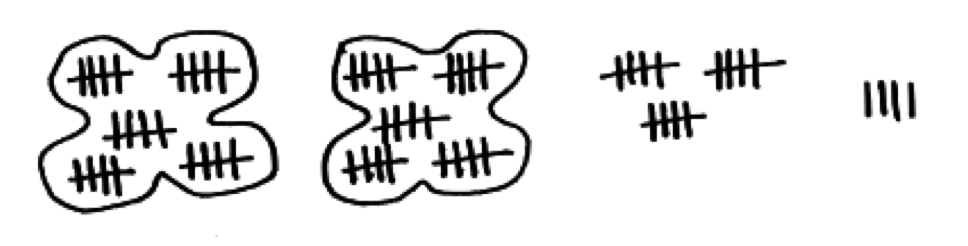
\includegraphics[height=0.75in]{lothar_goats.png}
\]
Lothar's wife, Gertrude, uses the following symbols to record things.
\[
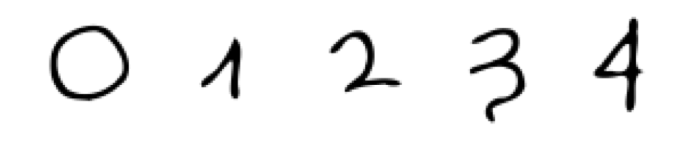
\includegraphics[height=0.4in]{gerturde_symbols.png}
\]
Gertrude writes the number of Lothar's goats as
\[
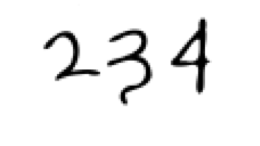
\includegraphics[height=0.4in]{gertrude_goats.png}
\]
In case it's helpful information, Gertrude would also write 5 goats as
\[
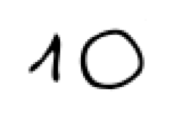
\includegraphics[height=0.4in]{gertrude_ex.png}
\]
Now answer the following questions about Gertrude's system.
\begin{problem}
If Lothar lost a goat, how would Gertrude write this new number of goats? 
\vfill
\end{problem}
\begin{problem}
If Lothar bought another goat (from the original number), how would Gertrude write this new number of goats? 
\vfill
\end{problem}
\begin{problem}
If we would write the number of goats as 37, how would Gertrude write the number of goats?
\vfill
\end{problem}
\begin{problem}
Explain the rules for Gertrude's counting system.  Write out a few (large) numbers in order as an example to show that you understand.
\vfill
\end{problem}


The aliens living on Omnicron Persei 8 keep track of how many humans they have eaten in the last week.  One such alien, Lrrr, tallies the number of humans he has eaten with this picture.
\[
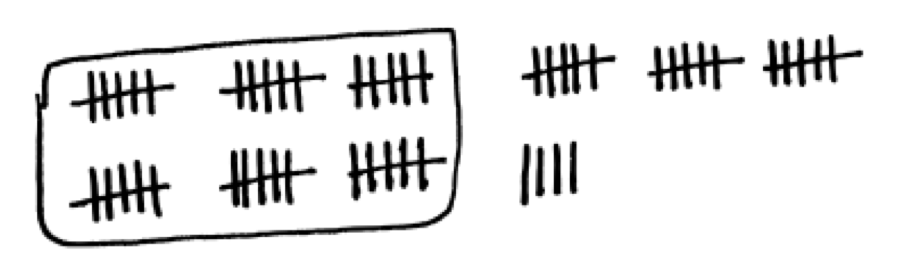
\includegraphics[height=0.75in]{omnicron_ate.png}
\]
His wife, Ndnd, uses the following symbols to write quantities.
\[

\includegraphics[height=0.4in]{omnicron_symbols.png}
\]
She writes the number of humans that Lrrr ate as follows.
\[
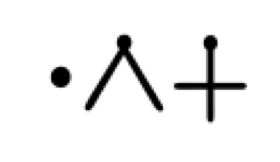
\includegraphics[height=0.4in]{omnicron_ate_again.png}
\]

\begin{problem}
If Lrrr ate another human, how would Ndnd write this new number of humans? 
\vfill
\end{problem}
\begin{problem}
If one of the humans actually escaped from the original number (and therefore was not eaten by Lrrr), how would Ndnd write this new number of humans? 
\vfill
\end{problem}
\begin{problem}
If we would write the number of humans as 101, how would Ndnd write this number?
\vfill
\end{problem}
\begin{problem}
Explain the rules for Ndnd's counting system.  Write out a few (large) numbers in order as an example to show that you understand.
\vfill
\end{problem}

\end{document}